\documentclass[12pt, twocolumn]{article}   	% use "amsart" instead of "article" for AMSLaTeX format
\setlength{\columnsep}{0.75cm}
\usepackage[ margin=2cm]{geometry}                		% See geometry.pdf to learn the layout options. There are lots.
\geometry{letterpaper}                   		% ... or a4paper or a5paper or ... 
%\geometry{landscape}                		% Activate for for rotated page geometry
\usepackage[parfill]{parskip}    		% Activate to begin paragraphs with an empty line rather than an indent
\usepackage{graphicx}				% Use pdf, png, jpg, or eps§ with pdflatex; use eps in DVI mode
								% TeX will automatically convert eps --> pdf in pdflatex		
\usepackage{amssymb}

\title{Cohort model to solve for the duration of infectiousness distribution }
\author{David Champredon}
%\date{}							% Activate to display a given date or no date

\newcommand{\K}{\mathcal{K}}
\newcommand{\eqref}[1]{(\ref{#1})}


\begin{document}
\maketitle

\section{Cohort model}

Consider an $SIR$ model with non-linear recovery:

\begin{eqnarray}
S' & = & \mu S - \beta SI \\
I' & = & \beta S I - \gamma I \K(I) \label{eq:dI}
\end{eqnarray}

Note that equation \eqref{eq:dI} can be rewritten as a per-capita rate of prevalence change
\begin{equation}
\frac{I(t)'}{I(t)}  =  \beta S(t)  - \gamma \K(I(t)) \label{eq:dIcapita}
\end{equation}
where the time dependence ($t>0$) has been explicitly made.

In order to find the expression of the duration of infectiousness distribution, we consider the cohort of individuals who acquired the disease at exactly time $\alpha>0$. Let's label the size of this cohort (as a proportion of the whole population) $c_\alpha$. This cohort is depleted at the same per-capita rate as the one given in equation \eqref{eq:dIcapita}. Hence, if $c_\alpha(\tau)$ is the size of this cohort $\tau$ units of time after disease acquisition, we have:

\begin{equation}
\frac{c_\alpha(\tau)'}{c_\alpha(\tau)}  =   - \gamma \K(I(\alpha+\tau)) \label{eq:c_alpha}
\end{equation}

The initial condition for $c_\alpha$ is theoretically arbitrary, and if we choose $c_\alpha(0)=1$, we can interpret $c_\alpha(\tau)$ as the probability of still being infectious $\tau$ units of time after having acquired the disease at time $\alpha$, in other words, the duration of infectiousness distribution.

Let's express \eqref{eq:c_alpha} with the original time variable $t = \alpha+\tau$:

\begin{equation}
\frac{c_\alpha(t-\alpha)'}{c_\alpha(t-\alpha)}  =   - \gamma \K(I(t)) \label{eq:c_alpha_t}
\end{equation}
and for convenience, let's introduce $p$ as
$$p_\alpha(t) = c_\alpha(t-\alpha)$$


The function $1-p_\alpha$ is the cumulative distribution of duration of infectiousness conditional on disease acquisition at time $\alpha$. It can be determined numerically by solving the following system:
\begin{eqnarray}
S' & = & \mu S - \beta SI \\
I' & = & \beta S I - \gamma I \K(I)\\ 
p_\alpha' & = & - \gamma p_\alpha\, \K(I) \label{eq:p_alpha}
\end{eqnarray}
with the initial conditions $I(0) = i_0$, $S(0)=1-i_0$ and $p_\alpha(\alpha)=1$. Note that $p_\alpha$ is not epidemiologically defined for $t<\alpha$, but it is nonetheless possible to arbitrary set $p_\alpha(t)=1$ for $t\leq \alpha$. Moreover, the density of the infectiousness duration is given by the derivative $-p_\alpha'$.

\section{Numerical solutions}

The right-hand side of equation \eqref{eq:p_alpha} is always negative, hence the distribution $p_\alpha$ is always decreasing. In particular, it cannot have a ``bumped'' shape (with a maximum at a positive time), that may be desirable in a epidemiological context. 

Figure \ref{fig:results} show the resulting distribution $p_\alpha$ for several $\alpha$ when solving numerically the ODEs. The simulations were run using:
\begin{itemize}
\item $R_0 = 2.0$
\item $\gamma = 1/4$
\item $\K(I) = (a+bI)^c$
\end{itemize}

The top panel is effectively a SIR model and we can verify that the distribution $p_\alpha$ is indeed an invariable exponential distribution (top centre panel, straight line on the log-scale) with a constant mean at $1/\gamma = 4$ days (top right panel).

Considering the second, third and fourth rows that depict $\K(I)=I^c$ with $c=0.5,1,2$ respectively, the centre panel confirms the convergence towards an exponential distribution (straight line on the log-scale) at equilibrium. Moreover, when using $\K(I)=I^c$ with $c>0$, the per-capita recovery rate is dramatically reduced (equation \eqref{eq:dIcapita}), increasing the length of the recovery: this is illustrated in the right panels, where the mean is very large as $c$ increases. 


\onecolumn

\begin{figure}[htpb]
\begin{center}
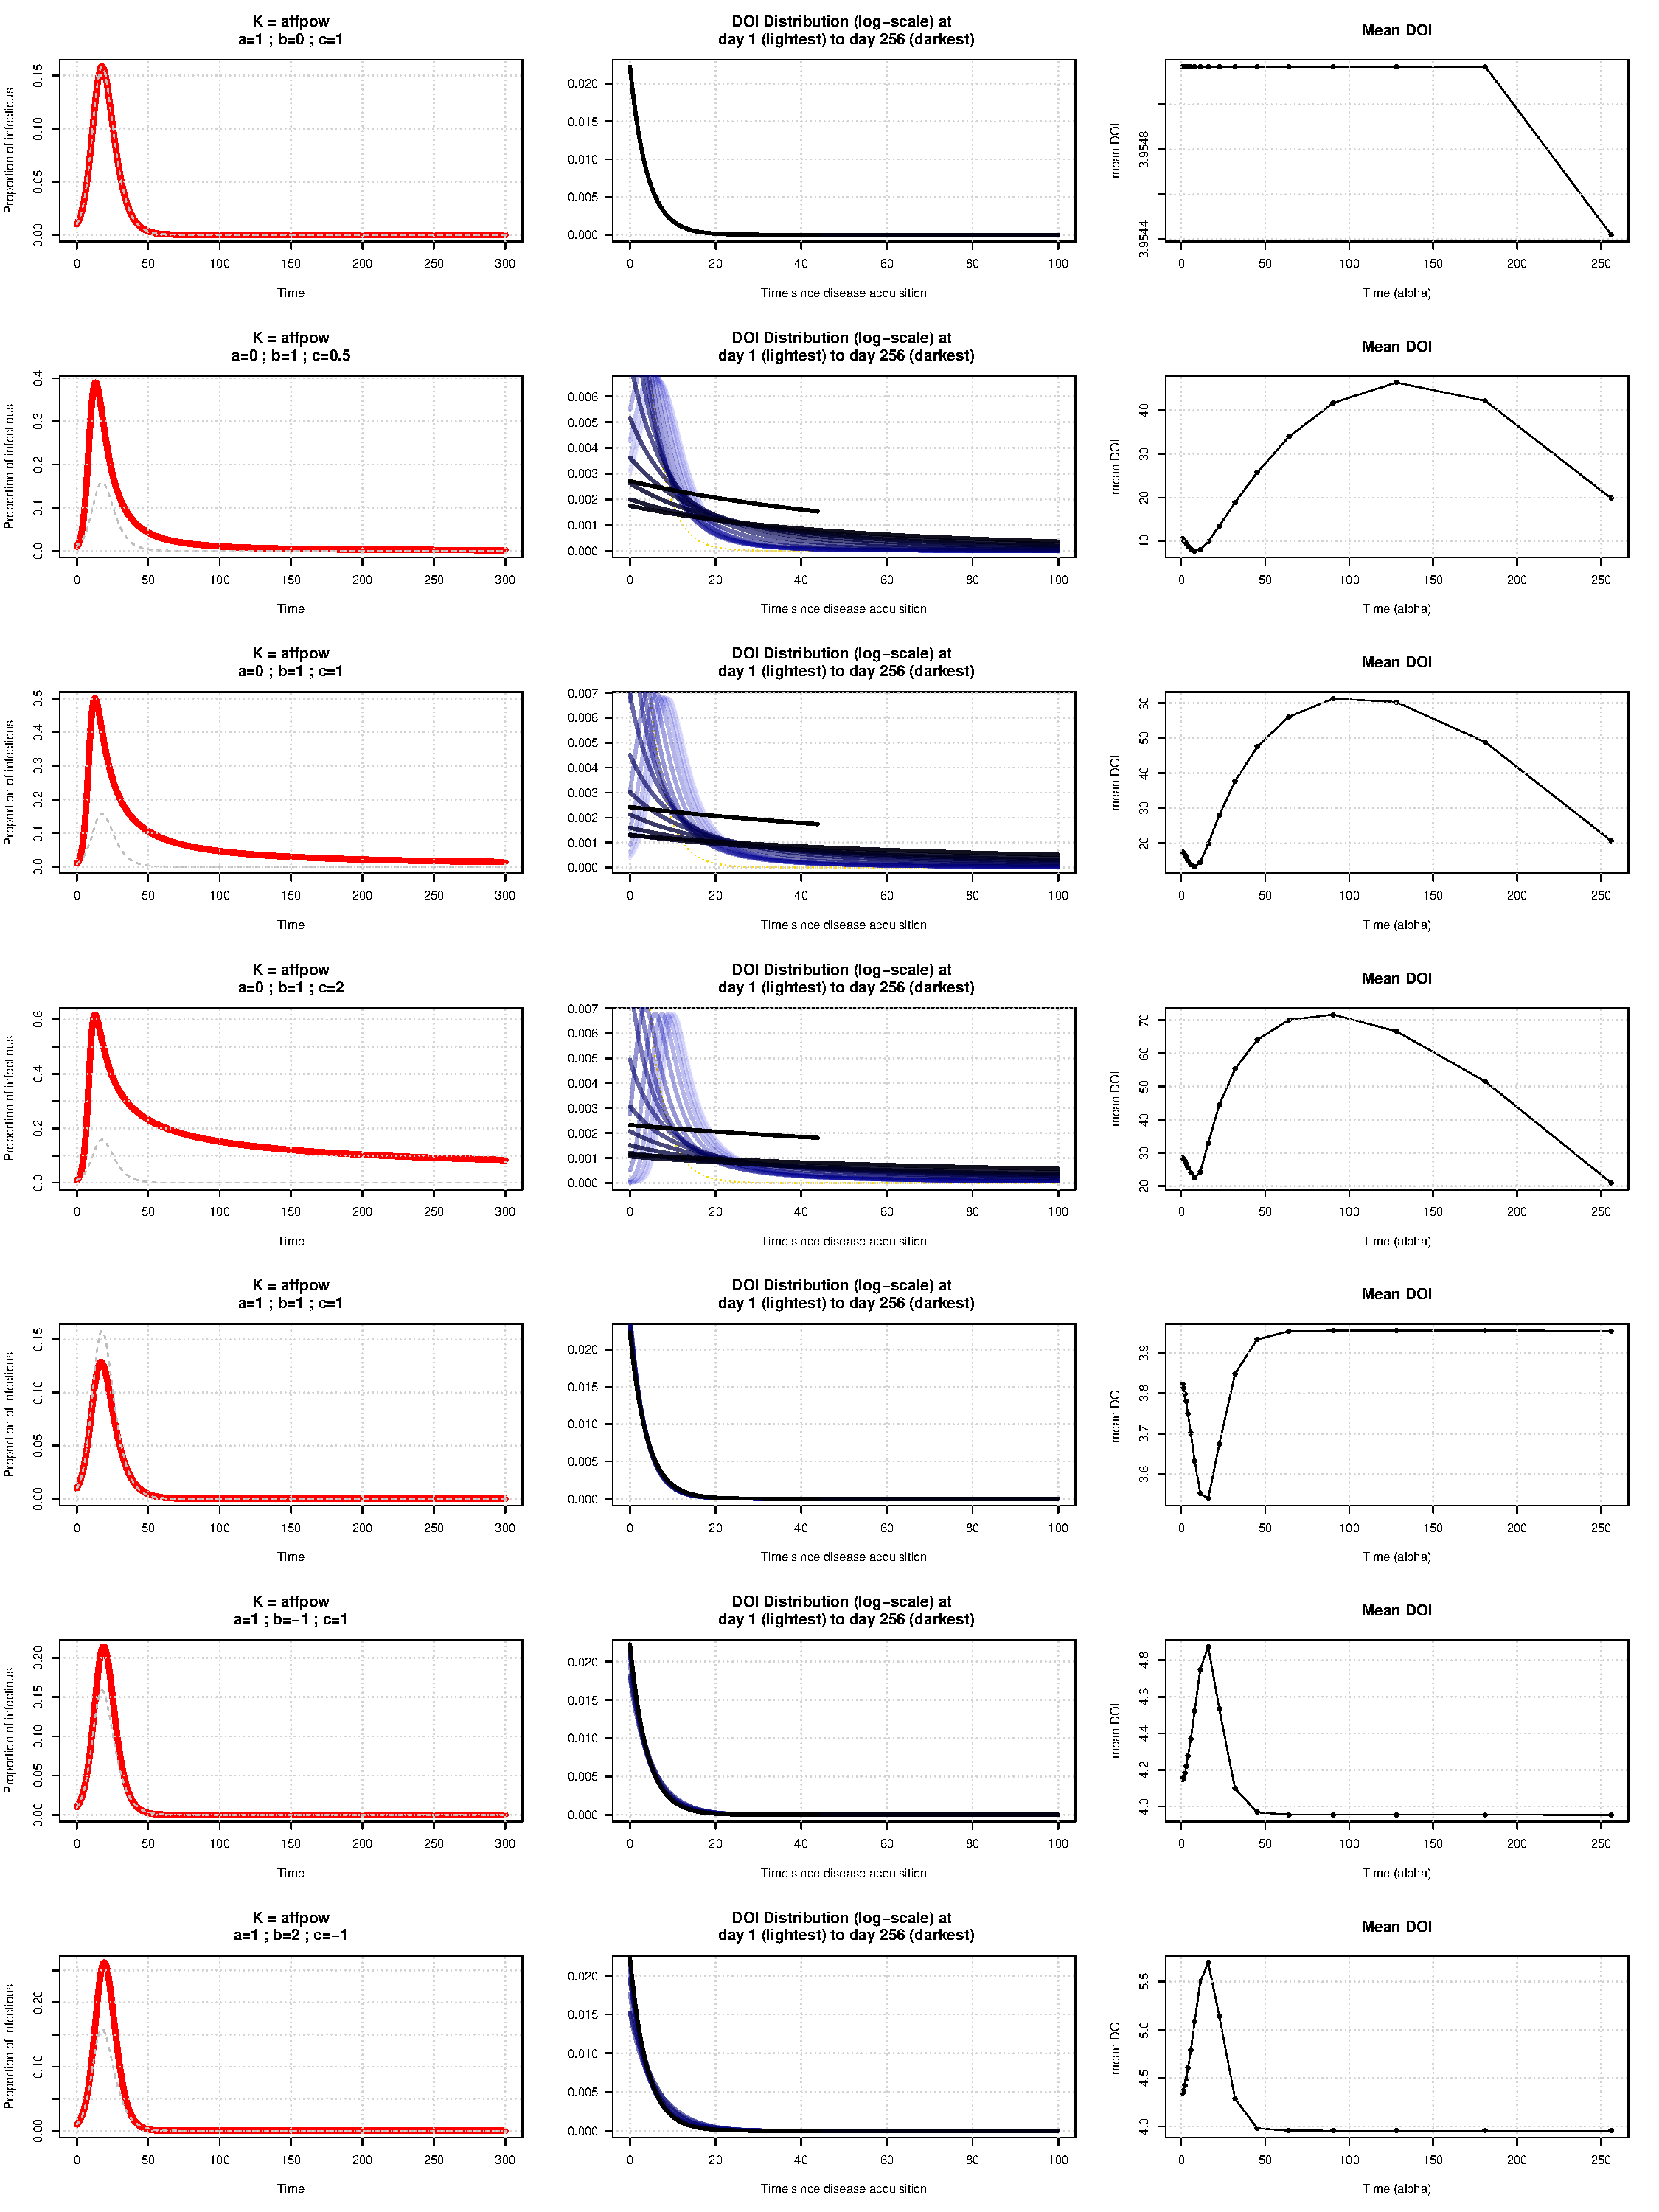
\includegraphics[width=0.9\textwidth]{plot_doid.pdf}

\caption{Left panels: time series of the proportion of infectious individuals (dashed line is to compare with the benchmark SIR model). Centre panels: distribution $p_\alpha$ (on the log-scale) for various values of $\alpha$. Right panels: mean of $p_\alpha$ (for the same given value of $\alpha$, each point is the mean of the distribution represented in the centre panel). See main text.}
\label{fig:results}
\end{center}
\end{figure}



\end{document}  